\documentclass{beamer}

%% Themes
%\usetheme{Madrid}
\usetheme{Berkeley}
%\usetheme{PaloAlto}
%\usetheme[left]{Marburg}
%\useoutertheme[left,height=0pt,width=0.12\paperwidth]{sidebar}
%\setbeamertemplate{sidebar canvas left}[vertical shading][top=black,bottom=blue]

%\usecolortheme[named=blue]{structure}

%% Beamer settings
\beamertemplatenavigationsymbolsempty  % Remove the navigation bar

%% Chinese environment
\usepackage[UTF8]{ctex}
%\usepackage{fontspec}
%\usepackage{xeCJK}
%\setCJKmainfont{SimSun}

%% Graphics
\usepackage{graphicx}
\usepackage{booktabs}   % Allows the use of \toprule, \midrule and \bottomrule in tables

\usepackage{caption} % Allow no-number caption of figures

%\usepackage[dvipsnames]{xcolor}
%\usepackage[sharp]{easylist} % Use # as \item

\setbeamertemplate{caption}[numbered]  % Add figure number

\title[]{序列密码算法电路的新型物理攻防技术研究}
% The short title appears at the bottom of every slide, the full title is only on the title page
\author[]{\texorpdfstring{导师:郭\quad 筝 \\ 学生:于泽汉}{}}
\institute[] % Your institution as it will appear on the bottom of every slide, may be shorthand to save space
{
    上海交通大学\quad 微纳电子学系 \\ % Your institution for the title page
}
\date{2018.01.11}


%% Show outline of current section before presenting details
\AtBeginSection[] % Do nothing for \section*
{
    \begin{frame}<beamer>
    \frametitle{}
    \tableofcontents[currentsection]
    \end{frame}
}
%\AtBeginSubsection[]
%{
%   \begin{frame}<beamer>
%   \frametitle{}
%   \tableofcontents[currentsection,currentsubsection]
%   \end{frame}
%}

% \setbeamerfont{normal text}{size=\fontsize{10}{4}} %, series=\bfseries}
\setbeamerfont{normal text}{size=\footnotesize} %, series=\bfseries}

\setbeamerfont{section in sidebar}{size=\fontsize{5}{4}\selectfont}
% \setbeamerfont{subsection in sidebar}{size=\fontsize{2}{4}\selectfont}
% \setbeamerfont{subsubsection in sidebar}{size=\fontsize{2}{4}\selectfont}

\setbeamerfont{itemize/enumerate body}{}
\setbeamerfont{itemize/enumerate subbody}{size=\scriptsize}
\setbeamerfont{itemize/enumerate subsubbody}{size=\tiny}

\setbeamerfont{caption}{size=\tiny}
% \setbeamerfont{caption name}{size=\tiny}

\AtBeginDocument{\usebeamerfont{normal text}}

\makeatletter
\beamer@headheight=2.5\baselineskip
\makeatother



% ppt提纲:
% 1、研究背景和意义(1-2页)
% 2、基础知识(别太多1-2页)
% 3、研究内容(重点、突出一些创新)
% (1)算法硬件实现
% (2)旁路分析方案
% 4、实验结果及分析
% 5、展望一些后续研究(1页)
% 不超过 20 页

\begin{document}

\begin{frame}
\titlepage
\end{frame}

\begin{frame}\frametitle{总览}
\tableofcontents
\end{frame}


% ------------------------------------ #
\section{研究背景和意义} % 1-2 页

\begin{frame}{祖冲之算法的历史和应用}
\begin{columns}
    \begin{column}{0.5\textwidth}
        
\includegraphics[width=0.8\columnwidth]{./images/lte.png}
    \end{column}
    \begin{column}{0.5\textwidth}
    \begin{itemize}
        \item 又称 ZUC 算法
        \item 我国自主研制
        \item 3GPP + LTE
        \item 序列密码算法
        \item 保护设备敏感信息
    \end{itemize}
    \end{column}
\end{columns}

\vspace{2\baselineskip}

经过多年的学术研究和工业应用,密码学理论已经日趋系统和完善,各种密码算法广泛应用于各种工业设备,以保障系统和数据的安全。

\vspace{0.5\baselineskip}

祖冲之算法是我国第一个成为国际密码标准的密码算法,在保障 4G 通信安全中起到了重要作用。
\end{frame}

\begin{frame}{旁路攻击对密码设备的威胁}

\begin{columns}
    \begin{column}{0.5\textwidth}
        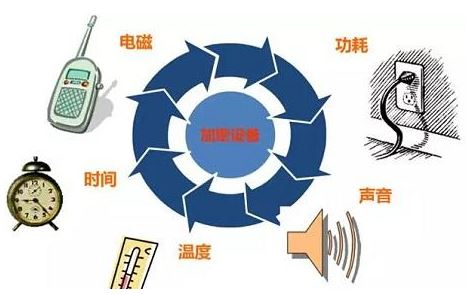
\includegraphics[width=\columnwidth]{./images/sca.jpg}
    \end{column}
    \begin{column}{0.5\textwidth}
        \begin{itemize}
            \item 理论安全 vs 实现漏洞
            \item 秘密信息泄露
            \item 功耗分析、电磁分析
            \item 威胁巨大
        \end{itemize}
    \end{column}
\end{columns}

\vspace{2\baselineskip}

目前,那些得到广泛使用的密码算法,通常都经过数学上的严格论证,并且经过了大量专家的研究和改进,因而在理论上基本是安全的。

\vspace{0.5\baselineskip}

然而在现实中,这些算法都运行在具体设备上,因此可能会暴露出许多安全问题,攻击者可以通过各种手段获取密码设备中的秘密信息。

\vspace{0.5\baselineskip}

因此,对祖冲之算法进行旁路分析,就有助于发掘其在实际设备上的漏洞,从而提出防护方案,提高密码设备的安全性。

\end{frame}

% ------------------------------------ #
\section{基础知识简介}   % 1-2 页

\begin{frame}{祖冲之算法的原理和流程}
\begin{columns}
    \begin{column}{0.5\textwidth}
        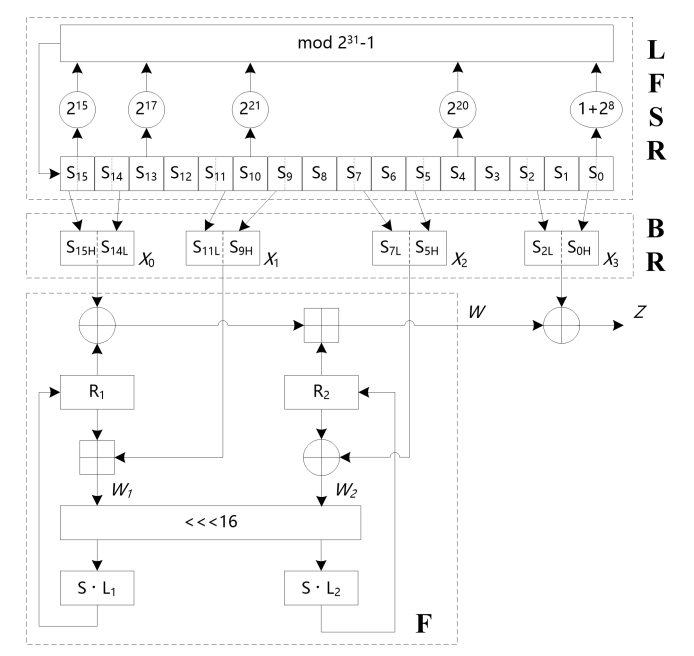
\includegraphics[width=\columnwidth]{./images/zuc-flow.png}
    \end{column}
    \begin{column}{0.5\textwidth}
        \begin{itemize}
            \item 三层结构
            \begin{itemize}
                \item 线性反馈移位寄存器
                \item 比特重组
                \item 非线性函数
            \end{itemize}
            \item 两种模式(LFSR)
            \begin{itemize}
                \item 初始化模式
                \item 工作模式
            \end{itemize}
            \item 两个阶段
            \begin{itemize}
                \item 初始化阶段
                \item 工作阶段
            \end{itemize}
        \end{itemize}
    \end{column}
\end{columns}
\end{frame}

\begin{frame}{差分功耗分析的一般流程}
\begin{columns}
    \begin{column}{0.45\textwidth}
        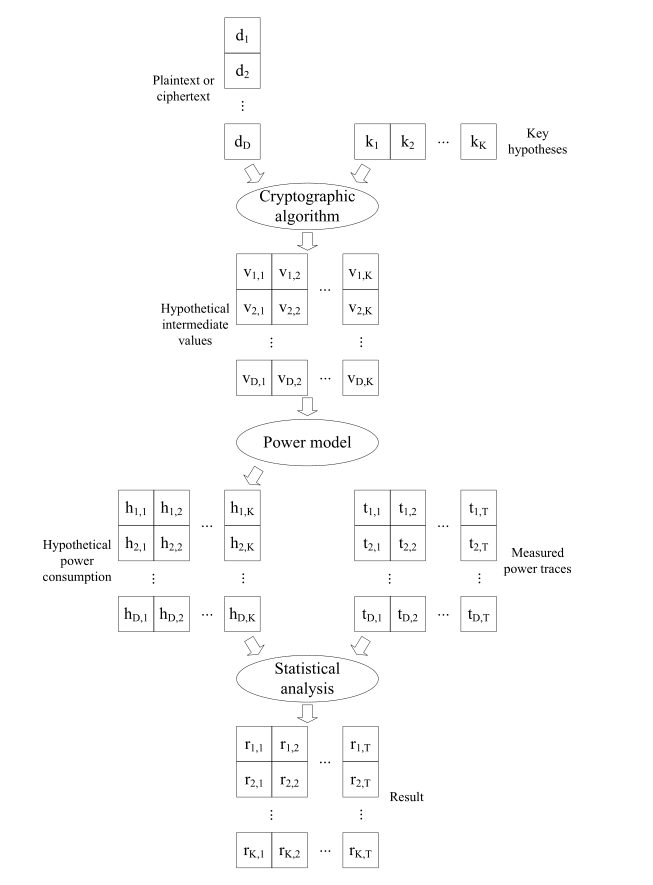
\includegraphics[width=\columnwidth]{./images/dpa.png}
    \end{column}
    \begin{column}{0.55\textwidth}
        \begin{itemize}
            \item 选取合适的算法中间值位置
            \item 采集设备运行时的实际功耗曲线
            \item 根据算法计算理论中间值
            \item 使用合适的功耗模型将理论中间值转换为假设功耗值
            \item 分析假设功耗值和实际功耗曲线,挖掘所需的信息
        \end{itemize}
    \end{column}
\end{columns}
\end{frame}


% ------------------------------------ #
\section{算法软硬件实现}

\begin{frame}{祖冲之算法的硬件实现}
硬件设计软件: ISE 14.3

FPGA 型号:XC6SLX75-2CSG484

\begin{columns}
    \begin{column}{0.4\textwidth}
        \begin{figure}[htbp]
            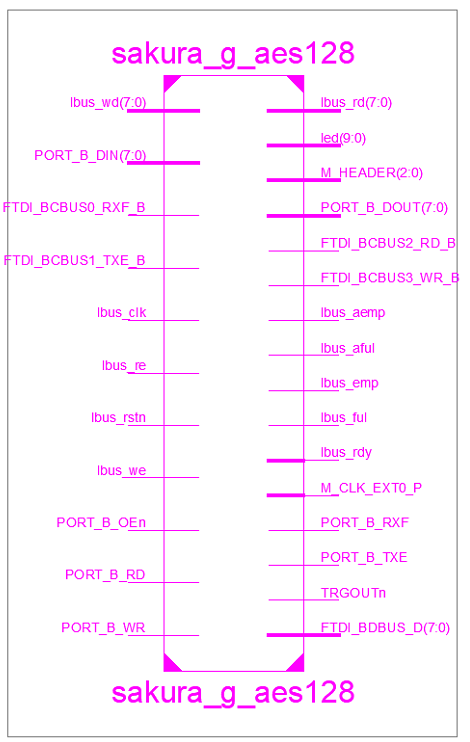
\includegraphics[height=0.6\textheight]{./images/circuit_io.png}
            \caption*{电路的输入和输出端口}
        \end{figure}
    \end{column}
    \begin{column}{0.6\textwidth}
        \begin{figure}[htbp]
            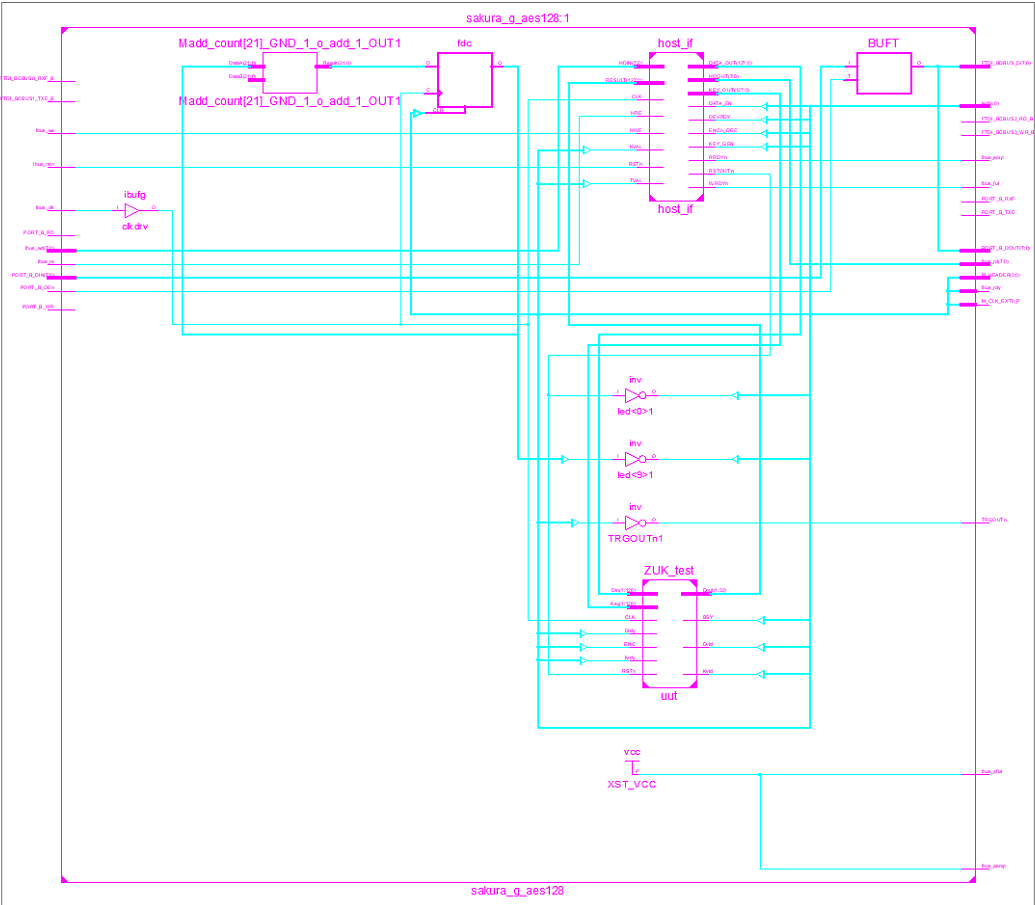
\includegraphics[height=0.6\textheight]{./images/circuit_more.png}
            \caption*{电路的内部结构}
        \end{figure}
    \end{column}
\end{columns}
\end{frame}

\begin{frame}{祖冲之算法的软件实现}
编程语言:Python 3.6

运行平台:Windows 10

\begin{columns}
    \begin{column}{0.5\textwidth}
        \begin{figure}[htbp]
            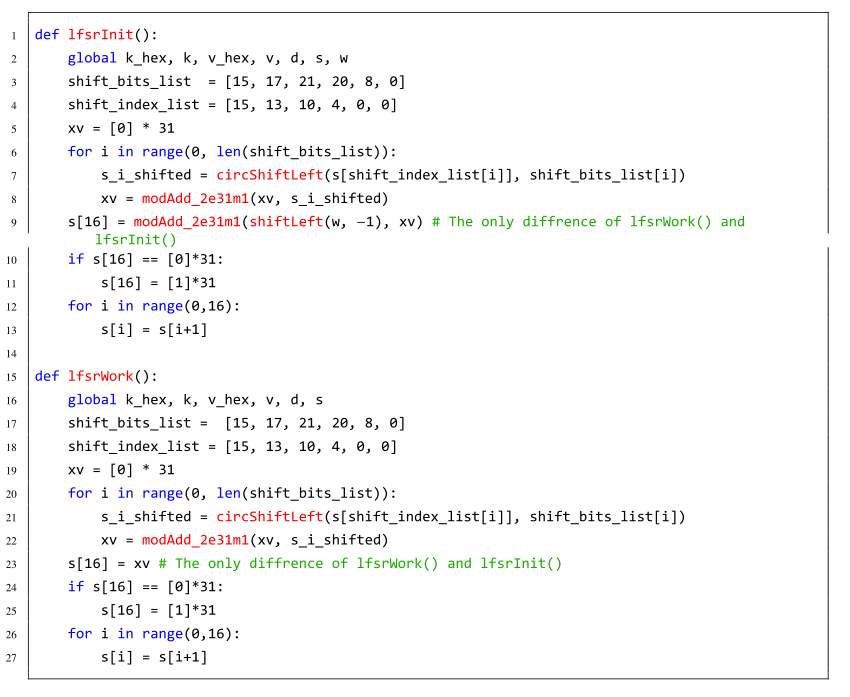
\includegraphics[width=\columnwidth]{./images/python_lfsr.png}
            \caption*{线性反馈移位寄存器模块}
        \end{figure}
    \end{column}
    \begin{column}{0.5\textwidth}
        \begin{figure}[htbp]
            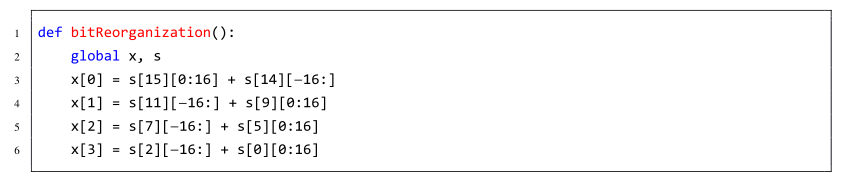
\includegraphics[width=\columnwidth]{./images/python_br.png}
            \caption*{比特重组模块}
        \end{figure}
        \begin{figure}[htbp]
            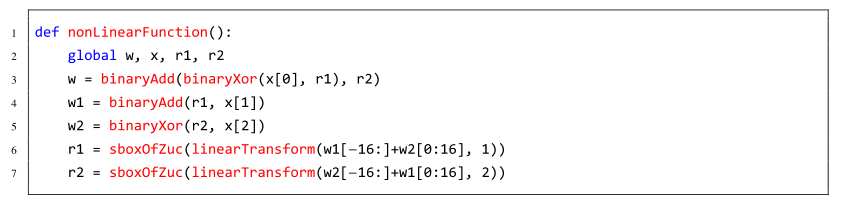
\includegraphics[width=\columnwidth]{./images/python_nf.png}
            \caption*{非线性函数模块}
        \end{figure}
    \end{column}
\end{columns}
\end{frame}

\begin{frame}{祖冲之算法的软件实现}

\end{frame}

% ------------------------------------ #
\section{功耗分析方案}




% ------------------------------------ #
\section{实验结果与分析}




% ------------------------------------ #
\section{后续研究展望} % 1 页




% ------------------------------------ #
\section{}
\begin{frame}{}
\centering \huge
\emph{谢谢!}
\end{frame}

\end{document}
